\chapter{Overview}

EMFText is a tool which allows to define a textual syntax for Ecore based
metamodels. From a specification of this syntax, EMFText generates
components to load, edit and store model instances. The syntax is specified 
by a so called concrete syntax specification which are stored in files with the
suffix \texttt{.cs}. A \texttt{cs} specification is directly related to one or 
more Ecore metamodel(s) which implicitly predefine a ''grammar skeleton''.
Figure~\ref{fig:overview} gives an overview on how the generator part of EMFText
works and which components are generated.

\begin{figure}
\centering
\ifpdf
	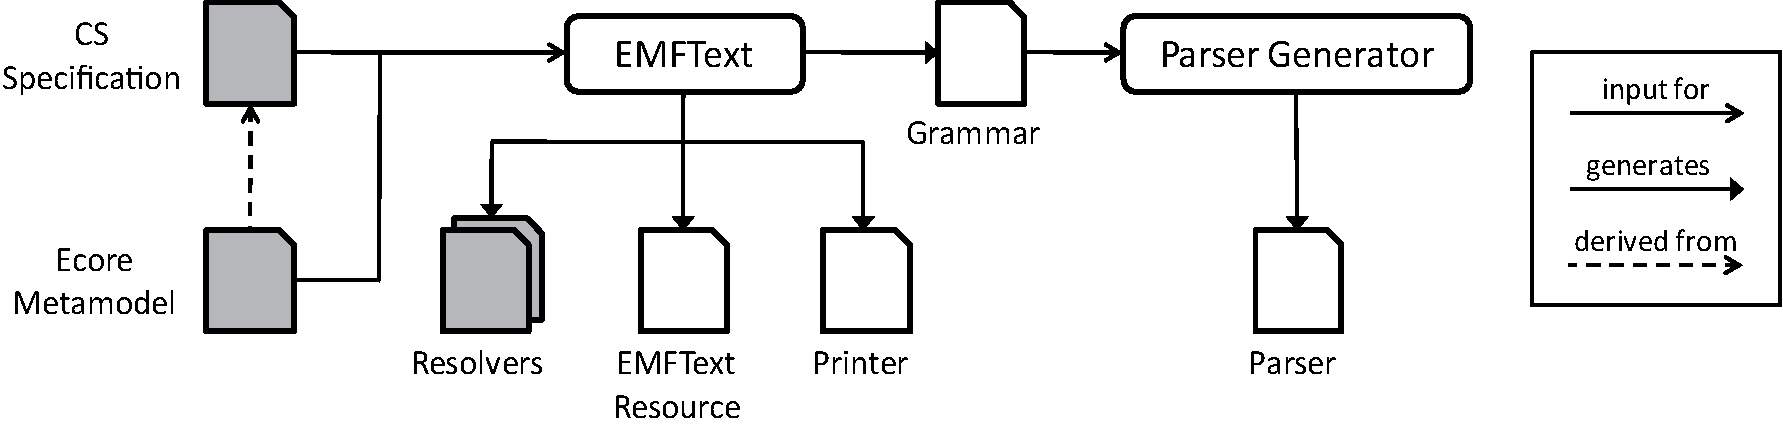
\includegraphics[width=1.0\textwidth]{../latex/figures/Overview.pdf}
\else
	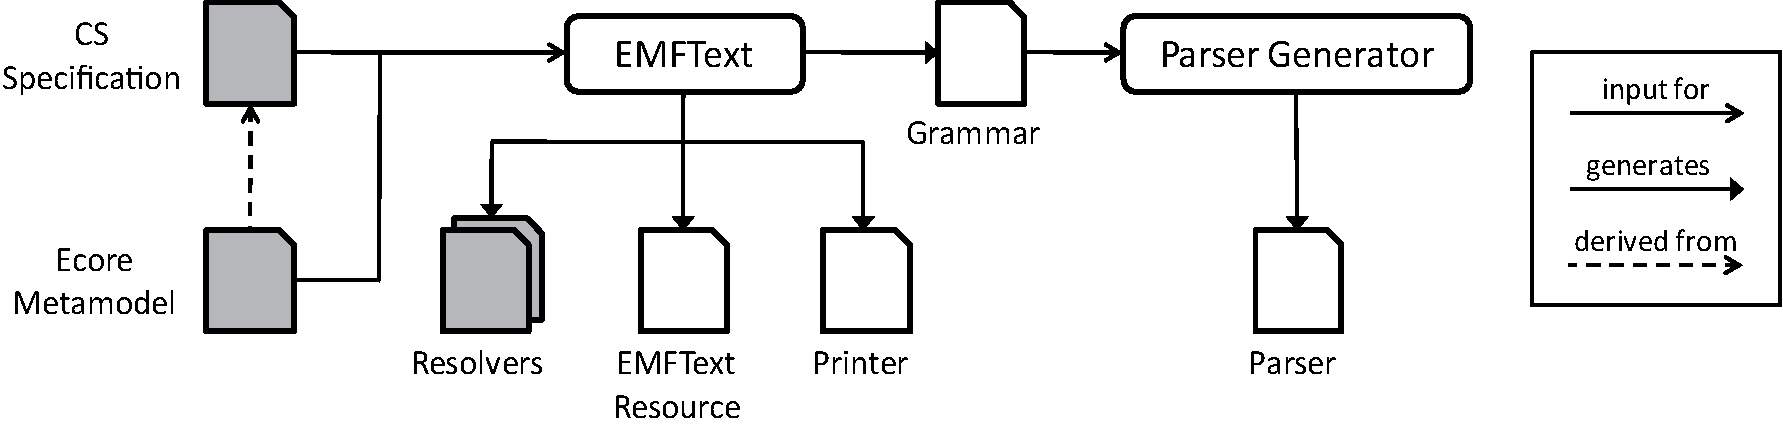
\includegraphics[width=1.0\textwidth]{../latex/figures/Overview.gif}
\fi
\caption{Overview of Specified and Generated Artefacts}
\label{fig:overview}
\end{figure}

Through combining metamodel and \texttt{cs} specification, EMFText derives a 
context-free grammar and exports it as an \ANTLR parser specification. This
specification contains annotated semantic actions which perform the
instantiation of models. EMFText then transparently delegates
parser\footnote{http://en.wikipedia.org/wiki/Parser} and 
lexer\footnote{http://en.wikipedia.org/wiki/Lexical\_analysis} generation to
\ANTLR by passing the generated grammar file. Since ANTLR does not cover the
whole class of context-free grammars one can not guarantee the generation of a
working parser for arbitrary cases. However, in most cases generation is
sufficient.

While parsers are used to load model instances from textual representations a 
printer is needed to do the inverse (e.g., to print an in-memory model)
back to a textual representation. The printed results can then 
again be parsed by the corresponding parser. Both instances (printed and
loaded) are be equal. Furthermore, printers produce a formatted and
human-readable output. The EMFText built-in printer generator achieves these
goals by interpreting the \texttt{cs} file and the derived grammar. 
Also, \texttt{cs} specifications can be enriched by 
special operators to indicate that on a specific position white-spaces or newlines 
have to be printed. Additionally, it uses information about literals (e.g.,
keywords) in defined languages which are removed from model instances. As for 
parser generation, EMFText does not guarantee that printer generation works for 
arbitrary cases but mostly it is be a convenient solution.

EMFText also generates a set of resolvers. Resolvers convert parsed token
strings to an adequate representation in the metamodel instance.

TokenResolvers implement a mapping from the string value of a specific token to a native 
Java type (e.g., boolean, int, String etc.). In the standard implementation
TokenResolvers can automatically remove and add (printing) pre- and suffixes. The conversion to native 
java data types is done by delegation to the corresponding Java type conversion
functions. For example, \texttt{Integer.parseInt("42")} results in an int valued
\texttt{42}. Since this behavior is only desired for concrete syntaxes
mirroring exactly (or at least partially) the Java syntax for primitive types, users are 
expected to implement more adequate mapping functions as needed.  

Resolvements depending on context are meant to be realised by implementing
ReferenceResolvers. For these only stubs are generated. While TokenResolvers are directly invoked by parsers, 
ReferenceResolvers are triggered on demand later by EMF's proxy resolution mechanism. An 
additional feature is the evaluation of eventually annotated \OCL constraints.
With \OCL, consistency conditions can be declared on the metamodel to further
improve quality of EMFText based developments.
